\chapter{The Genetic Basis of Variation}
\label{cha:genetic-basis-of-variation}
\index{Environment and heredity|(}
\index{Nonadditive interactions of heredity and environment|(}
\index{Variation!genetic basis of|(}

Variation --- differences between individuals --- is the raw material on
which the breeder works. It is not necessary that the animals vary widely
enough that the breeder can at the very start find some perfect ones
to select, but merely that some of them will be closer to his ideal than
others are.

The causes of variation are differences in the heredity with which
individuals started life, and differences in the environments, internal
and external, known and unknown, to which they were exposed during
their development. Except in the case of identical twins\index{Identical twins}, two individuals
rarely if ever start with all their genes identical.\footnote{In organisms
which can reproduce asexually, (as many plants can by cuttings, budding,
etc.,) large groups of individuals with identical heredity can occur. These
are called ``clones.'' A highly inbred line either of plants or animals,
also approaches the condition in which all individuals in it have the same
heredity, but this approach is asymptotic and it is rarely if ever possible
to be sure that complete identity of heredity has been reached. The broad
term, ``isogenic line,''\index{Isogenic lines} which includes identical twins, clones, and
completely inbred lines, is convenient where it is desired only to mean that
all members of the group have identical heredity, regardless of how that
group was produced.} No two individuals ever develop under absolutely
identical environments. Hence in practice an observed difference between two
individuals must always be considered as the net result of some differences
in their heredity and some differences in their environment. Hereditary and
environmental differences may have been far from equal in the size of the
effects they produced, but almost always both will have been present. They may
have opposed each other or both may have worked in the same direction.

Besides these two main divisions of variation into hereditary and
environmental portions, a third portion (necessary for logical completeness)
comes from joint effects of heredity and environment which cannot fairly be
ascribed to either one alone. Such joint effects may occur either if heredity
and environment are correlated or if they interact in some nonadditive way so
that the effect of a particular variation in heredity may be larger in one
environment than in another or, conversely, a certain change in environment
may make a large change in individuals of some genotypes but only a small
change in other individuals whose genotypes make them less labile.

Positive correlation between heredity and environment makes the
whole population more variable by preventing the plus effects of variations
in heredity from being canceled in individual animals by the
minus effects of variations in environment, or vice versa, as often as
would be the case if the two were uncorrelated. Such a correlation is an
ever-present possibility in data which are collected from a variety of
farms, since it often happens that the man who tries hardest to give his
animals the best environment also tries hardest to select the animals
with the best heredity and has some degree of success in both efforts.
Correlation between heredity and environment is also likely to exist in
data concerning the mental and social traits of man, since inherited
aptitudes on the part of the parents tend to cause them to create in their
own homes environments which favor the development of those same
special abilities in their children. These children will also inherit some
of the same genes which made those parents have those aptitudes in the
first place.

It seems likely that the nonadditive combination effects of heredity
and environment are generally small in amount,\footnote{For some extreme
examples, consult Chapter 5 of Hogben's \textit{Nature and Nurture}.}
but some interactions of this kind do occur.
\index{Environment and heredity|)}
\index{Nonadditive interactions of heredity and environment|)}

\section*{MODES OF GENE EXPRESSION}
\index{Additive effects of genes|(}

The simplest way in which the effects of various genes are combined
is that the substitution of a gene for its allel produces a certain plus or
minus shift in the measurement of the characteristic affected and that
this change --- the ``effect'' of that gene substitution --- is the same, regardless
of what other genes are present. As a physical example, consider
how adding or subtracting one more brick makes exactly the same
increase or decrease in the weight of a brick pile, regardless of the number
or kind of bricks the pile already contains. Some genes may combine
their effects exactly in this simple way and many seem to do so to some
extent, yet many genes are known to interact with each other so that the
outward result of substituting a gene for its allel is larger in some genotypes
and smaller or zero or even reversed in other genotypes. Thus the
actual effect of the gene substitution in each separate individual may
depend partly on what other genes are present.

A simple example is \index{Dominance|(}dominance. If dominance exists, the outward
effect of substituting gene \textit{A} for \textit{a} is larger when the
substitution is made in an individual which is \textit{aa} than when it
is made in one which is \textit{Aa}, although the effect on breeding value
of the individual is the same; namely, that it now transmits \textit{A} to
one-half of its offspring which would otherwise have received \textit{a}
from it. Dominance is nonadditive combination of the effects of genes which
are in the same allelic series. When the effect of making two such gene
substitutions in an \textit{aa} individual is not simply twice as large as
the effect of one, some degree of dominance exists.

\index{Epistatic effects|(}
Genes which are not allelic may also modify the magnitude or even the
direction of each other's effects. A classic example is Bateson's case of
white and purple flowers in sweet peas. He found that two different pairs of
genes, both showing dominance, were necessary for the production of the purple
color. Plants which were \textit{cc} had white flowers, no matter whether they
were \textit{RR}, \textit{Rr}, or \textit{rr}; and plants which were \textit{rr}
had white flowers, no matter whether they were \textit{CC}, \textit{Cc}, or
\textit{cc}. But plants which were either \textit{CC} or \textit{Cc} and were also
\textit{RR} or \textit{Rr} had purple flowers. It is as if \textit{R} produced an
enzyme necessary for developing color and \textit{C} produced the substrate on which
the enzyme could work. Whether the substitution of \textit{C} for \textit{c} will
produce a change from white to purple depends on whether \textit{R} is also present,
as well as on whether the substitution is made in a \textit{cc} or in a \textit{Cc}
individual. The difference between purple and white is a joint effect the credit or
blame for which cannot wholly be divided fairly, part to one gene and the rest to the
other. An example in which the direction of the effect depends on other genes is the
case of the \textit{E} gene in guinea pigs, which darkens certain colors in the presence
of the \textit{P} gene but lightens them in \textit{pp} individuals. Many other kinds of
nonadditive combinations of the effects of genes are known. Some common examples are:
inhibiting genes, threshold effects\index{Threshold effects}, and the general class of cases in which the outward
extreme is genetically an intermediate. The latter may be very common among physiologically
complex characteristics where the degree of expression of the characteristic depends on
the harmonious interplay of a number of different organs and processes.

\section*{SUBDIVISION OF HEREDITARY VARIATION}

In an actual population there will be genes acting in all these ways,
and the number of genes and possible kinds of interactions between
them is so enormous that there is no possibility of learning exactly
what each gene does in every combination. The simplest way to think
of this tangled situation is to imagine that one could average the effects
(some of them large, some small, some positive, some negative, etc.)
which a gene substitution actually does have in that particular population
and then proceed as if this \textit{average effect} were the \textit{actual
effect} of that gene substitution in all genotypes and under all environmental
circumstances which occur in that population. In effect this is what we do
when we speak of a gene as ``good'' or ``bad,'' or as ``a gene for high
production.''

By adding these average effects of all the genes which an animal has
we can obtain an ``expected'' value, or measurement of the appearance
or individual performance of this animal. The expected and the actual
characteristics may not be exactly the same, if the genes interact in
nonadditive ways. The expected value of an individual corresponds more
closely to its breeding value than its own appearance or performance
does.

The variation of the expected values from each other is the additively
genetic portion of the actual variation. Differences between the
expected and the actual values are deviations from the simple additive
scheme. It is convenient to divide these nonadditive deviations into two
groups, the first being the deviations caused by dominance and the second
being the nonadditive interactions of genes which are not allelic
to each other. For brevity these latter are called ``epistatic'' deviations
in this book, although this is a broader use of epistatic than Bateson
intended when he introduced the word.

To understand the principles of what we do when we separate the
additively genetic variation from that due to dominance deviations,
consider the two cases shown in Figure~\ref{fig:Lush_Figure_6}. Polled is
considered a simple dominant over horns in cattle.\footnote{This fits most
of the facts as far as yet known, but there are a few sets of data in which
the situation seems more complicated. Also dominance is not always complete,
scurs being some indication of heterozygosis.} The frequencies of the three
genotypes in this example were assumed to be: \textit{PP}, .01; \textit{Pp},
.18; and \textit{pp}, .81. These are not far from the present frequencies of
the three types in the Hereford breed as a whole in the United States.
Probably there actually are slightly more \textit{PP} and fewer \textit{Pp}
individuals than this.

The actual or phenotypic values are indicated by Y's and the expected or
genetic or breeding values are indicated by G's. The G values come nearer
to agreeing with the Y values than could any other three values which lie on
a straight line.\footnote{The \textit{G} values must lie on a straight line
since they are made to conform to the assumption of no dominance; i.e., the
phenotypic change expected from substituting \textit{P} for \textit{p} is to
be the same when the substitution is made in \textit{Pp} individuals as when
it is made in \textit{pp} individuals. The \textit{G} values are completely
determined by the requirement that the sum of the squares of their deviations
from the \textit{Y} values shall be the least possible for any set of three
values which are on a straight line. This is the ``least squares'' method for
fitting a straight line as closely as possible to observations which do not
actually lie on a straight line.} In technical statistical terms, the line
connecting the \textit{G} values shows the regression of phenotypic values on
breeding values. If there were no dominance $Y_{Pp}$ would lie on a straight
line connecting $Y_{pp}$ and $Y_{PP}$ and the \textit{G} values would fit the
\textit{Y} values exactly. Hence the discrepancies between each \textit{G} and
the corresponding \textit{Y} (on the vertical scale) are called dominance
deviations. Vertical differences between the G values are the additively genetic
deviations. If we let the difference between horned and polled be one unit on
the vertical scale, we can compare on a quantitative basis the additively
genetic variation and the dominance deviations and find how important both are.
We get the following values:

\begin{table}[htbp]
	\centering
	\begin{tabular}{lccc}
		Genotype				& \textit{pp}	& \textit{Pp}	& \textit{PP} \\
		Frequency				& $.81$			& $.18$			& $.01$ \\
		Actual phenotype, Y		& $y$			& $y+1.00$		& $y+1.00$ \\
		G value					& $y+.01$		& $y+.91$		& $y+1.81$ \\
		Y--G					& $-.01$		& $.09$			& $-.81$ \\
	\end{tabular}
\end{table}

\noindent
When we summarize the variation in terms of ``variance''\index{Variance|(} {(See
page \pageref{page79}) we find that 18/19 of the actual variation is included in the
variation of the G values, while only 1/19 of it has to be charged against
the dominance deviations. In this case the additive scheme comes near to telling
all the truth, even though dominance is complete. The G values are far apart and
the variation between them is large. The discrepancy between G and Y is very
small for the \textit{pp} genotype which includes most of the individuals. Nearly
all the rest of the individuals are in the \textit{Pp} group where the dominance
deviation is also rather small. The dominance deviation is large for the
\textit{PP} group, but the \textit{PP} animals are rare and hence contribute only
a few deviations to the total and do not have much influence.

\begin{figure}
	\centering
    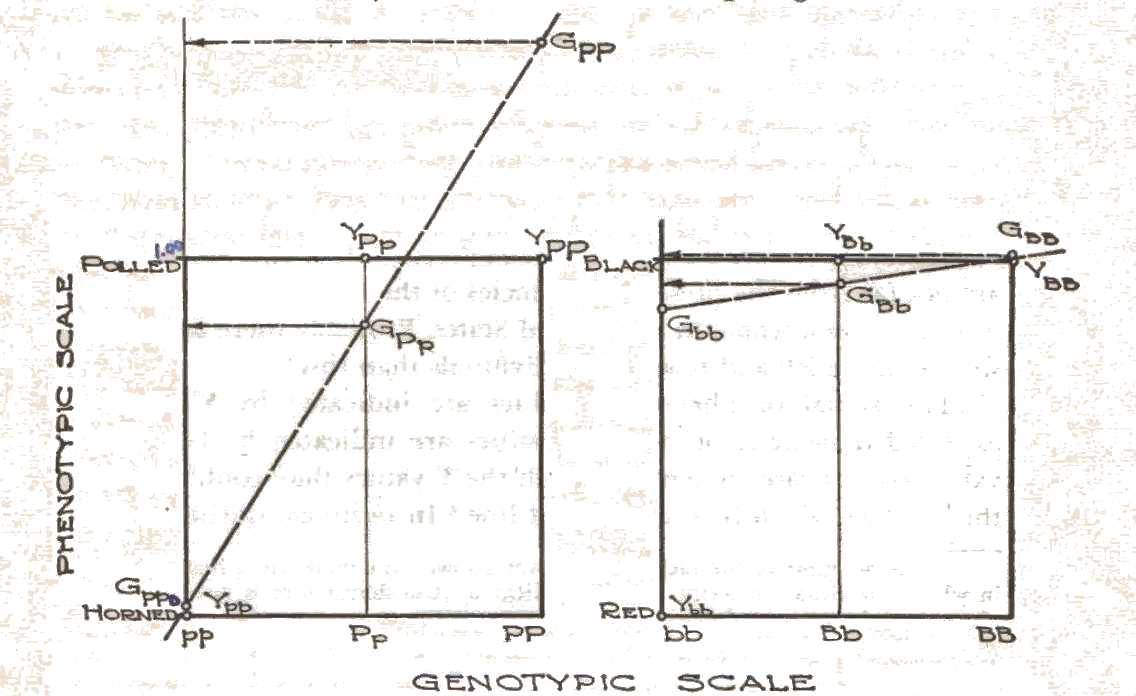
\includegraphics[width=\textwidth]{Figure_6.png}
    \caption{Diagram of regression of phenotype on genotype where only additively
    		 genetic variance and dominance deviations arc involved. Left: A case
    		 where the dominant is rare, the G-values arc far apart, and most of
    		 the variance is additive. Right: A case where the recessive is rare
    		 and the dominance deviations cause much more variance than the
    		 differences between G-values.}
    \label{fig:Lush_Figure_6}
\end{figure}

The average effect of substituting \textit{P} for \textit{p} may be computed as
follows: For every 100 individuals in the population there will be 180 \textit{p}
genes and 20 \textit{P} genes. Of the \textit{p} genes 18 are in \textit{Pp}
individuals where changing them to \textit{P} would produce no phenotypic effect.
The other 162 are in \textit{pp} individuals and for any one of these a change to
\textit{P} would change the phenotype of its possessor one full unit. Hence the
average effect of substituting \textit{P} for \textit{p} in this particular population
would be $\frac{162}{180} = .9$ unit.\footnote{This simple arithmetical way of
computing the average effect illustrates its meaning and will be correct when the
\index{Heterozygosis}heterozygotes are present in the same proportion as they would be under random mating.
When they are more abundant or less abundant than that, the average effect should he
computed by the more technical procedure which is called the least squares method of
fitting a straight line.}

Obviously, the size of the average effect and the comparative importance
of additive and dominance variations will depend on the frequency
of the genotypes, as well as on the degree of dominance. These are
part of the description of this particular population.

The right side of \ref{fig:Lush_Figure_6} shows for comparison how different the
situation is when the recessive is very rare. The \textit{Bb} pair of genes
determines the contrast between black and red in cattle, black being completely
dominant. The frequencies assumed for the genotypes are about what they would be
in black breeds of cattle in which one calf in each 200 is born red. The actual
variation is small and the variation between the G values accounts for on1y
$\frac{14}{107}$ of it. Dominance deviations account for the rest, $\frac{93}{107}$.
The contrast between the left and the right sides of \ref{fig:Lush_Figure_6}
illustrates the general fact (of which more in \textbf{\textit{Chapter 11}}) that
dominance is an \textit{important} source of confusion or hindrance to progress by selection
only when the undesired recessive is already rare. Even when dominance is complete,
the variance among the G values will account for $\frac{2(1-q)}{2-q}$ of the actual
variance\label{page79} in random breeding populations, \textit{q} being the frequency of the
dominant gene.
\index{Variance|)}

For a numerical example of epistatic variance, let us take again the
case of purple and white flowers in sweet peas. Its genetic basis is definite
and well-known, and it is generally considered to be a rather
extreme case of epistasis -- although that idea may need revision when
we learn more about the usual results of making several gene substitutions
at one time. If the sweet peas were breeding at random,\footnote{The sweet pea does
not really fulfill this condition, since it is largely self-fertilizing.} and if the
frequencies of the \textit{C} gene and of the \textit{R} gene were each .5, then
the various genotypes would occur in the proportions shown in column 1 of
Table~\ref{tbl:Lush_Table_5}.

\begin{table}[htbp]
	\centering
	\caption{\textsc{Illustration of the Basis for Separating Additive Genetic Variations, From
			 Deviations Caused by Dominance and Epistasis, Using Bateson's Case of Purple
			 and White Color in Sweet Peas}}
	\label{tbl:Lush_Table_5}
	\begin{tabular}{C{2cm}|C{2cm}|C{1.25cm}|C{2cm}|C{2.25cm}}
		\hline
		\hline
					& & \multicolumn{3}{C{6cm}}{Values on a Scale on Which White = 0 and Purple = 1} \\
		\cline{3-5}
		Frequency With Which the Various Genotypes Would Occur	& Fraction of the \textit{e} Genes of the Whole Population Which Are in This Genotype & Actual	& ``Expected''	& Deviations Due to Dominance and Epistasis \\
 		\hline
		1 ccrr	& $1/8$	& 0	& $-3/16$	& $+3/16$ \\
		2 Ccrr	& $2/8$	& 0	& $+3/16$	& $-3/16$ \\  
		2 ccRr	& $2/8$	& 0	& $+3/16$	& $-3/16$ \\
		1 CCrr	& none	& 0	& $+9/15$	& $-9/16$ \\
		1 ccRR	& $1/8$	& 0	& $+9/16$	& $-9/16$ \\
		4 CcRr	& $2/8$	& 1	& $+9/16$	& $+7/16$ \\
		2 CcRR	& $1/8$	& 1	& $+15/16$	& $+1/16$ \\
		2 CCRr	& none	& 1	& $+15/16$	& $+1/16$ \\
		1 CCRR	& none	& 1	& $+21/16$	& $-5/16$ \\
 		\hline
	\end{tabular}
\end{table}

If we let the difference between purple and white be one unit on the scale on which
we measure color, then in this population the average effect of substituting
\textit{C} for \textit{c} is $3/8$ of a unit. That may be computed as follows:
One-half of all the \textit{c} genes are in \textit{Cc} individuals (the second,
sixth, and seventh lines in Table~\ref{tbl:Lush_Table_5}), where, on account of
dominance, the substitution would make no change in the color. One-eighth of the
\textit{c} genes are in \textit{ccrr} individuals (the first line in
Table~\ref{tbl:Lush_Table_5}), where the substitution would produce no outward effect
because the \textit{R} gene, which is also necessary for the production of purple, is
not present. The remaining three-eighth of the \textit{c} genes are in \textit{ccRR}
or \textit{ccRr} individuals, where the substitution of \textit{C} for \textit{c}
would produce the full change from white to purple. One unit of change in three-eighths
of the cases plus no change in five-eighths of the cases makes an average effect of
three-eighths of a unit for substituting \textit{C} for \textit{c} in that population,
although the actual change would not be exactly three-eighths of a unit in any one
plant.\footnote{For a more detailed discussion of this conception of the average effect of a
gene substitution, see the first few pages of Wright's article beginning on p. 243 of
volume 30 of the \textit{Jour. of Genetics}, or pages 53--56 in volume 11 of
\textit{Annals of Eugenics}, 1941.} The expected values shown in Table~\ref{tbl:Lush_Table_5}
were found by the additional requirement that the average of the expected values must
be the same as the average of the actual values. Figure 7 shows graphically how near the
actual and the ``expected'' values are to each other. The differences between them (the last
column in Table~\ref{tbl:Lush_Table_5}) are the deviations caused jointly by dominance and
epistasis.

\begin{figure}
	\centering
    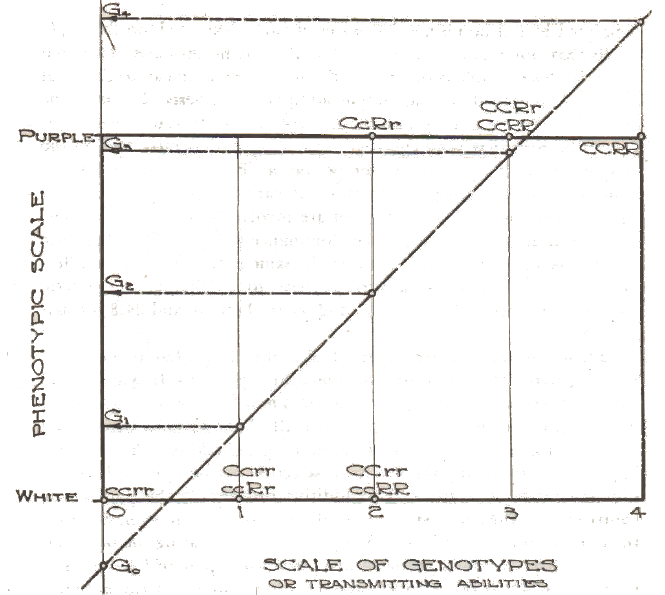
\includegraphics[width=\textwidth]{Figure_7.png}
    \caption{Regression of phenotypes on transmitting ability in a case involving epistatic
			 deviations in addition to dominance deviations and additive differences.
			 $G_0 \cdots G_4$ are the expected values or transmitting abilities of
			 individuals which have $0, 1, \cdots, 4$; respectively, of the \textit{C}
			 and \textit{R} genes. Differences (on the vertical scale) between the
			\textit{G} values are the additive variation. Differences (on the vertical
			scale) between each \textit{G} value and the corresponding actual value are
			deviations caused by dominance and epistasis together.}
    \label{fig:Lush_Figure_7}
\end{figure}

\index{Variance|(}
Variance due to dominance and variance due to epistasis can be
separated by setting up another series of values expected, on the hypothesis
that dominance is complete but there is no epistasis. The final
result in this example is that $4/7$ of the actual variation can be gathered
into and described by the simple additive hypothesis, $2/7$ must be
charged to dominance deviations, and only $1/7$ to epistatic deviations.
It will be seen that the expected values are partly determined by the
frequencies with which the genotypes occur. They are partial descriptions
of a particular population and may vary from one population to
another, even where the same genes are involved. The relative importance
of additive genetic variance, dominance deviations, and epistatic
deviations will change also. Thus, in the same example but with different
gene frequencies the ratio of additive to dominance to epistatic
variance becomes 12:9:2 when $q_R$ and $q_0$ are both .6, and 24:8:9 when
both are .4.

These illustrations are intended to make clear what is meant by
dividing hereditary variation into these three portions. In actual practice
the breeder or investigator will not know exactly what genes are
present, nor the frequency of each, nor all of the ways in which they
interact with each other. Rough estimates of the additive variance can
be had from observing the results of selection or the likeness between
different kinds of relatives. The additive variation is the part which
contributes in the simplest and most direct way to the likeness between
relatives. Knowledge of its size is important for estimating the probable
results of any proposed breeding plan. For many practical purposes it
may not be worth while to separate the dominance and the epistatic
portions from each other.

The additive genetic variation caused by a gene can become zero
only when the average effect of that gene is zero; that is, when the sum
of all the plus changes which it causes is exactly equal to the sum of all
the minus changes which it causes in other genotypes in that same
population. Most of the variation which a gene causes will be included
in the additive portion if its average effect is large. For most of its variation
to be epistatic requires that its average effect be near zero but that
it produce large plus effects in some genotypes and correspondingly
large minus effects in other genotypes. As yet there are only a few actual
data to indicate whether epistatic variations are abundant and important,
or so rare and small that ignoring them in practice would not
cause many errors.\index{Additive effects of genes|)}
\index{Dominance|)}
\index{Epistatic effects|)}

\section*{THE MEASUREMENT OF VARIATION}
\index{Variation!measurement of}

The methods of measuring variation are inconveniently technical for those not
trained in statistical methods. Moreover, there are several of them, and each
has advantages for certain purposes. For reasons which do not concern us here,
the importance of various causes in producing the variability of a population is
most conveniently expressed in terms of the ``variance'' ($\sigma^2$) of that
population. The variance may be defined as the average of the squared deviations
of the individuals from the population average.\footnote{Since the known average
of the \textit{n} individuals in the sample studied may not be exactly the same as
the unknown average of the much larger population from which the sample comes, the
sum of the \textit{n} squared deviations of individuals from the average of the
sample is divided by $n - 1$ instead of \textit{n} to obtain the best estimate of
the variance of the population.} An equivalent definition is that the variance is
one-half of the average squared difference between pairs of individuals chosen at
random. The square root of the variance is called the ``standard deviation''\index{Standard deviation}
($\sigma$), which, since it is expressed in the same terms as the original
measurements, is often more convenient for expressing the variations of individual
items than is the variance, which is expressed in squares of the original
measurements. In a ``normally distributed'' population about two-thirds of the
individuals differ from the average by less than the standard deviation, while
about one-sixth of the individuals will be more than one standard deviation above
the average. The remaining sixth will be below the average by more than one standard
deviation. Only about one-fortieth of the individuals will be more than twice the
standard deviation above the average and another fortieth will be more than twice
the standard deviation below the average. In small populations the standard
deviation is usually about one-fourth to one-sixth of the difference between the
largest and the smallest individuals (the ``range''); but that rule is not very
accurate, since the range depends on only two individuals and is subject to large
sampling errors. The arithmetic average of the deviations, neglecting signs, is
about .8 as large as $\sigma$, but for various reasons is not as dependable and is almost
never used.
\index{Variance|)}

\index{Normal distributions|(}
Not all populations are ``normally'' distributed, although most of
those encountered in breeding practice are nearly enough so that the
statistics of the normal curve may be used with little error for practical
purposes. The normal curve is frequently called the ``Gaussian curve''
after the mathematician who first studied it in detail, or the ``curve of
error'' because its first application, which is still its principal application
in some sciences, was in making allowance for unavoidable but
random errors of observation. It is symmetrical and bell-shaped, as will
be seen in Figure~\ref{fig:Lush_Figure_8}.

\begin{figure}
    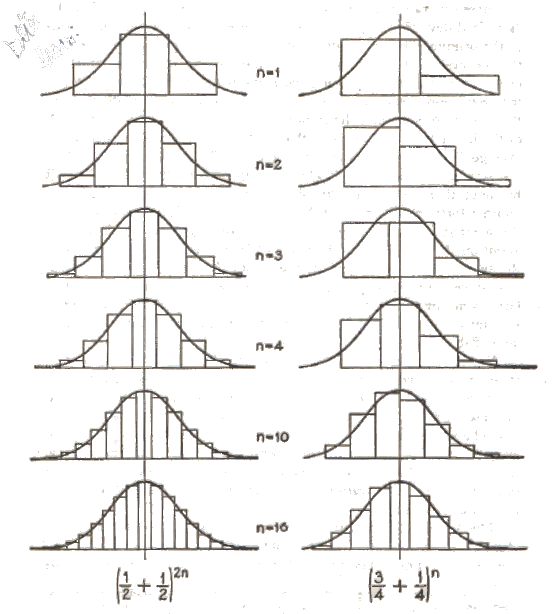
\includegraphics[width=\textwidth]{Figure_8.png}
    \caption{Binomial distributions for \textit{n} pairs of genes with equal effects
    		 and superposed normal curves with equal mean, equal area, and equal
    		 variance. Left: No dominance. Right: Complete dominance in the same
    		 direction in all pairs of genes.}
    \label{fig:Lush_Figure_8}
\end{figure}

\index{Binomial distribution|(}
The statistical cornerstone for the genetics of populations is the
``binomial distribution,'' which is obtained by expanding the expression
$(a + b)^n$. This is just the mathematical description of what results
naturally from the duplicateness of inheritance and the ``one-or-otherness''
of gene transmission; that is, of Mendel's laws of segregation and
recombination. \index{Dominance|(}The Mendelian mechanism guarantees that in a random-
mating\index{Random mating|(} population the zygotes\index{Zygotic ratios|(} will be distributed according to the
square of the gametic ratio. The genotypes for characteristics determined
by \textit{n} pairs of genes\index{Variation!as affected by gene numbers} with equal frequencies and equal effects will
have the binomial distribution corresponding to $[qA + (1 - q)a]^{2n}$.
If the gene frequencies are not the same for all pairs of genes, the
distribution will be somewhat less variable than if they were all equal but
had the same average. If the different pairs of genes do not have equal
effects, the distribution of the genotypes is more variable than if the
same number of genes each played equal parts in producing the same
total effect. When $a = b$ (or $q = 1 - q$ in the genetic formula) and
\textit{n} is large, the binomial distribution approaches the normal
distribution so closely that for practical purposes they may be treated alike,
especially in small populations. The binomial curve can be distinctly skewed
to one side if all of the genes which operate in the plus direction happen
to be much more frequent than their alleles, or the reverse . It can also be
skewed if the genes multiply each other's effects instead of combining additively,
or if there are threshold or other epistatic interactions.
Figure~\ref{fig:Lush_Figure_8} shows on the left side several symmetrical
binomial curves with normal curves superposed on them. With some additional
environmental modifications to blur the accuracy of classification, the binomial
curve, even with very small values of n, could not be surely distinguished from
the normal curve in small populations. The right side of Figure 8 shows how the
skewness produced by dominance, even when the dominance is all in one direction,
is extreme when \textit{n} is small butwould be difficult to detect in small
populations if there were as many as 10 pairs of genes involve d, especially if
there were also many variations from environmental causes.
\index{Binomial distribution|)}
\index{Dominance|)}
\index{Normal distributions|)}

\index{``Blending inheritance''|(}
\index{Variance|(}
\index{Variation!maintained by Mendelian mechanism|(}
One of the most important consequences of the Mendelian mechanism of inheritance
is that it maintains the variability of an interbreeding opulation at a nearly
constant level over long periods of time, thus aintaining a supply of variability
available for selection or other reeding practices. The importance of this may be
shown most clearly y contrasting it with what would be expected under the blending
theory of inheritance. Under that theory, if the sire deviated \textit{x} and the
dam deviated \textit{y} from the mean of the race, \textit{every} offspring from
that mating would be expected to deviate $\frac{x + y}{2}$ The average squared
deviation (the variance) of the parents would be $\frac{x^2 + y^2}{2}$. The average
squared deviation of the offspring would be $\frac{x^2 + 2xy + y^2}{4}$. If the
parents mated at random, sires with positive values of \textit{x} having no especial
tendency to mate with dams which had positive values of \textit{y}, the term
\textit{2xy} would be zero (since the negative terms would cancel the positive
ones); and the average squared deviation of each generation would be \textit{only
half as large as that of the preceding one}. The group would thus  approach perfect
uniformity at a tremendous rate. Even a pronounced tendency for like to mate with
like would delay this approach only a little (by causing \textit{2xy} to have a
positive value) unless the tendency of like to mate with like were perfect.
Figure~\ref{fig:Lush_Figure_9} shows how rapidly the hereditary variability
existing at any one time would be ``swamped'' if inheritance really were blending,
and how much of the hereditary variability existing at any one moment must have
come from mutations which had just occurred in the last few generations, if the
variability of a population were to remain the same from generation to generation.
Much of the skepticism about Darwin's theory of evolution by natural selection had
its roots in the tacit assumption that inheritance is ``blending'' and the consequent
belief that selection would have to be almost instant and perfect in its seizure of
new variations if these were to be incorporated into the species before they were
lost. In the older view, heredity was a conserving force and variation was contradictory
to it. That is now obsolete as it is seen that the mechanism of heredity conserves
individual variation also. Knowledge of Mendelism and of the hereditary variation to be
expected between full brothers has freed us from the supposed necessity of thinking that
mutations are frequent or important in practical breeding problems. It has also relieved
us from the necessity of believing that selection must act almost at once if it is to
utilize variations before they are ``swamped'' or lost. In many respects Mendelism has
rounded out the Darwinian theory of the power of natural selection by showing that some
of its us supposed weaknesses do not exist.\footnote{See pp. 1--12 of Fisher's
\textit{The Genetical Theory of Natural Selection}.}

\begin{figure}
    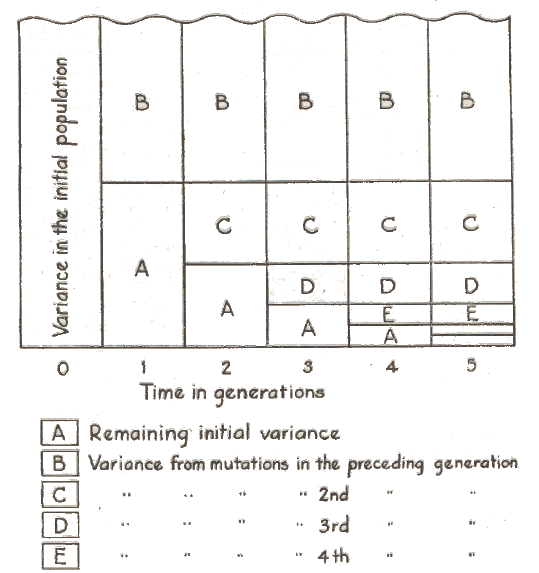
\includegraphics[width=\textwidth]{Figure_9.png}
    \caption{Rate at which initial hereditary variance was supposed to be lost and the
			 supposed recent origin of the hereditary variations existing at any one time,
			 according to the former theory that inheritance really blended.}
    \label{fig:Lush_Figure_9}
    \index{Random mating|)}
    \index{Variance|)}
\end{figure}

Mendelism gives us a picture of a stable population composed of
changing individuals, or of endless individual variations which added
together result in an almost constant population. A Mendelian population
may be compared to a group of bees around a hive. Almost every
bee is constantly in motion and yet the average position of the swarm
may remain almost the same hour after hour. The individuals are
dynamic -- the population is almost static. Changing a population by
selection may be compared roughly to driving a herd of many hundred
steers. At any one time there are steers moving in all possible directions,
yet the drivers, by constantly discouraging those which attempt to move
toward the rear and leaving the road open to those which go in the
desired direction, can succeed in moving the herd a few miles each day.
\index{``Blending inheritance''|)}
\index{Variation!maintained by Mendelian mechanism|)}
\index{Zygotic ratios|)}

The \textit{Correlation coefficient|(} is a measure of how closely two things
tend to vary in the same direction. Examples are the tendency in human
data for father and son both to be tall or both to be short and the tendency
for tall men to weigh more than short men. In both cases the
tendency is pronounced enough that it is a matter of common knowledge,
even to those who have never heard it expressed quantitatively. In
both cases there are frequent and striking exceptions. In the former
case the measurements are the same kind (i.e., stature), and they are
paired together on account of the genetic relationship of their possessors.
In the latter case the measurements (i.e., stature and weight) are
different in kind and are paired together because they apply to the same
individual. The general idea of correlation is simple and universally
understood, but the coefficient for measuring degrees of correlation is
technical enough that considerable practice in computing it on
various kinds of data is usually necessary for proficiency in understanding
it. The coefficient of correlation is expressed on a scale running
from $+1.0$, where two characteristics vary in perfect step with each
other, through zero, where there is no correspondence at all, to $-1.0$,
where there is a perfect tendency to vary in exactly opposite directions
from each other.

\index{Regression|(}
\textit{Regression} is the general statistical term for expressing how much
one variable may be expected to change per unit change in some other
variable. As a concrete example, in dairy cattle regression of daughter's
fat yield on dam's fat yield is the average amount of increase in the fat
production of the daughter which we may expect for each extra unit of
fat the dam produced. Historically regression gets its name from acertain
aspect of correlation wherein it was observed that the offspring of
extreme parents are usually nearer to the average of the population
than their parents were; i.e., they regress toward the mean of the race.
This idea of regression of the offspring from the parents toward the
mean of the race was later extended to all kinds of equations for predicting
one variable from another, where the relation between the two
is not perfect. Regression is now used in many cases which do not
involve questions of heredity at all and even in cases where the idea of
the correlation coefficient would be artificial, as in time trends. The customary
symbol for the correlation coefficient, r, was originally chosen
because it was the first letter of the word regression. Thus, it is a
reminder of the once intimate relation between the two ideas!

\section*{SUMMARY}

Variation is the raw material with which the breeder works. For
purposes of subdivision into its constituent parts, variation is best measured
in terms of ``variance,'' which is the average squared deviation of
the individuals from the population average. According to its causes,
variance may be divided into three main parts: that due to variations in
environment ($\sigma_E^2$), that due to differences in heredity ($\sigma_H^2$), and that
due to joint effects of variations in heredity and environment ($\sigma_{HE}^2$)
which are nonadditive or othenvise intertangled so that they cannot
fairly be ascribed to heredity or to environment alone. The hereditary
variance may be further subdivided into three portions: the additive
genetic variance, which includes all that can be described by assuming
that the effects of the whole combination of genes in the individual
equal the sum of the average effects of those genes ($\sigma_G^2$); the variance
caused by dominance deviations from the additive scheme ($\sigma_D^2$); and
the variance caused by epistatic deviations from the additive scheme
($\sigma_I^2$).

For expressing the variation of individuals, or for expressing differences
between expected and actual values, variation is most conveniently
expressed in the form of the standard deviation ($\sigma$), which is the
square root of the variance. In most populations about two-thirds of
the individuals differ from the population average by less than the
standard deviation.

The tendency for two different characteristics of the same individual,
or for the same characteristic in pairs of individuals related in a certain
way, to vary in the same direction is measured by the ``coefficient
of correlation.'' The equation for predicting the value of one characteristic
which will most probably correspond with a given value of
another characteristic is called a ``regression'' equation.
\index{Correlation coefficient|)}
\index{Regression|)}
\index{Variation!genetic basis of|)}
\index{Variation!measurement of|)}